\section{Floats}
This section goes over tables and figures.

\begin{figure}[H] % H forces figure to be here exactly
	\centering
	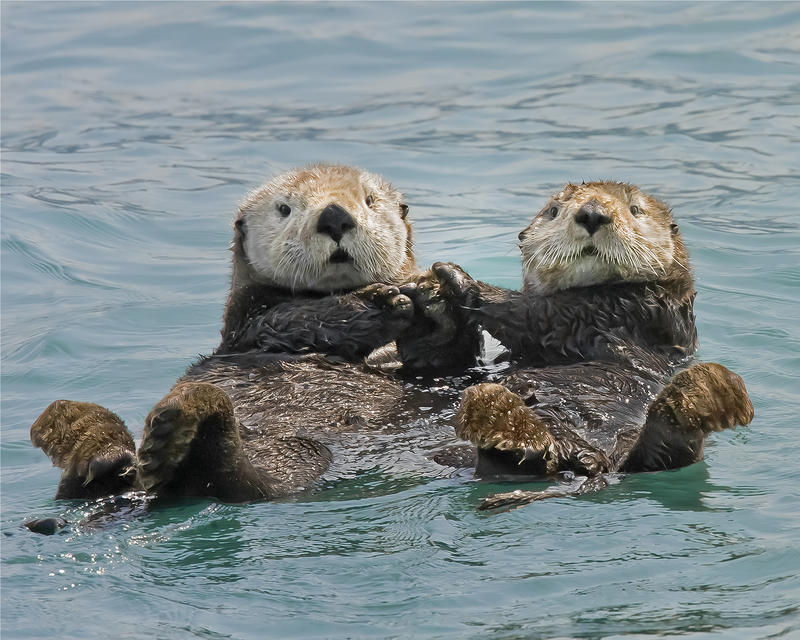
\includegraphics[width=0.7\textwidth]{sea_otters_holding_hands_by_ken_conger.jpg}
	\caption{Sea OTTURS Holding Hands}
	\label{fig:sealion}
\end{figure}

Here, otturs are holding hands \ref{fig:sealion}

In the table, we can see that seaotturs are simply superior
\begin{table}[H]
	\centering
	\begin{tabular}{||c c c c||} 
		\hline
		Fish & Sealions & Seaotturs & Magic \\ [0.5ex] 
		\hline\hline
		1 & 6 & 87837 & $\omega$ \\ 
		2 & 7 & 78 & $\Omega$  \\
		3 & 545 & 778 & $\delta$  \\
		4 & 545 & 18744 & $\alpha$  \\
		5 & 88 & 788 & $\beta$  \\ [1ex] 
		\hline
	\end{tabular}
	\caption{Table to test captions and labels. \cite{Otturs2020}}
	\label{table:1}
\end{table}

And this table we can clearly see seaotturs just goign crazy

In the table, we can see that seaotturs are simply superior
\begin{table}[H]
	\centering
	\begin{tabular}{||c c c c||} 
		\hline
		Fish & Sealions & Seaotturs & Magic \\ 
		\hline\hline
		1 & 6 & $\infty$ & $\omega$ \\ 
		2 & 7 & $\infty$ & $\Omega$  \\
		3 & 545 & $\infty$ & $\delta$  \\
		4 & 545 & $\infty$ & $\alpha$  \\
		5 & 88 & $\infty$ & $\beta$  \\
		\hline
	\end{tabular}
	\caption{Table to test captions and labels. \cite{Otturs2020}}
	\label{table:2}
\end{table}
